\documentclass{article}

\usepackage[brazil]{babel}
\usepackage{listings}
\usepackage{fontspec}
\usepackage{graphicx}
\usepackage{multicol}
\usepackage{geometry}
\geometry{a4paper, left = 20mm, right = 40mm, top = 20mm}

\title{Modelagem e Simulação - INE 5425\\
Programa de Simulação em Linguagem de Propósito Geral}

\author{Evandro Chagas Ribeiro da Rosa}

\begin{document}

\maketitle

\section{Manual}
A interface de usuário é dividida em 3 partes.

\subsection{Configuração}
\begin{multicols}{2}
  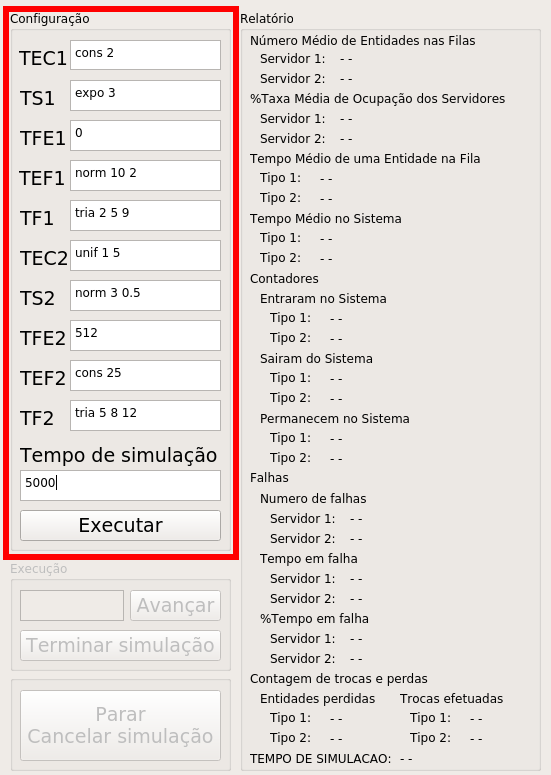
\includegraphics[width=0.4\textwidth]{imgs/conf.png}
\columnbreak

Aqui são configurados todos os parâmetros da simulação. Os parâmetros que podem receber uma
  função de probabilidade devem corresponder com os seguintes padrões:
\begin{itemize}
  \item \texttt{expo media}: Exponencial.
  \item \texttt{norm media dp}: Normal.
  \item \texttt{tria min moda max}: Triangular
  \item \texttt{unif min max} : Uniforme;
  \item \texttt{cons valor}: retorna sempre valor.
\end{itemize}
Usar `` . '' ao invés  de `` , '' para separa a parte inteira da fracionaria.
\end{multicols}

Siglas:
\begin{itemize}
  \item TEC1: Tempo entre chegadas do Servidor 1.
  \item TS1: Tempo de serviço do Servidor 1.
  \item TFE1: Tamanho da fila de entrada do servidor 1, 0 significa ilimitado.
  \item TEF1: Tempo entre falhas do Servidor 1.
  \item TF1: Tempo de falha do Servidor 1
  \item TEC2: Tempo entre chegadas do Servidor 2.
  \item TS2: Tempo de serviço do Servidor 2.
  \item TFE2: Tamanho da fila de entrada do servidor 2, 0 significa ilimitado.
  \item TEF2: Tempo entre falhas do Servidor 2.
  \item TF2: Tempo de falha do Servidor 2
\end{itemize}

Apos tudo configurado clique em ``Executar'' para começar a simulação.

\subsection{Execução}
\begin{multicols}{2}
  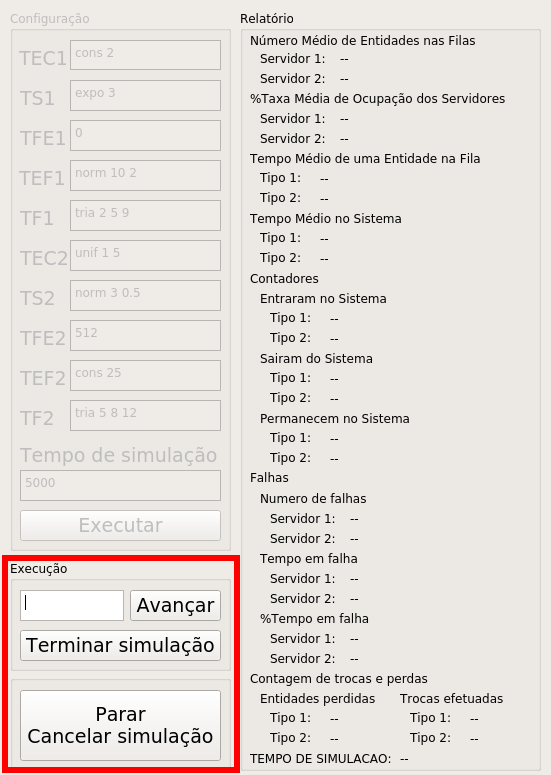
\includegraphics[width=0.4\textwidth]{imgs/run.png}
\columnbreak

Essa parte será usado durante a simulação. 
\begin{itemize}
  \item Botão ``Avançar'': Avança a simulação no tempo conforme especificado na caixa de texto a esquerda (usar apenas numero separado por `` . '' ao invés de `` , ''). 
  \item Botão ``Terminar Simulação'': Executa a simulação até o final.
  \item Botão ``Parar / Cancelar Simulação'': Para o avanço da simulação, caso já esteja
    parada cancela a simulação liberando a parte de configuração.
\end{itemize}

\end{multicols}

\subsection{Relatório}
\begin{multicols}{2}
  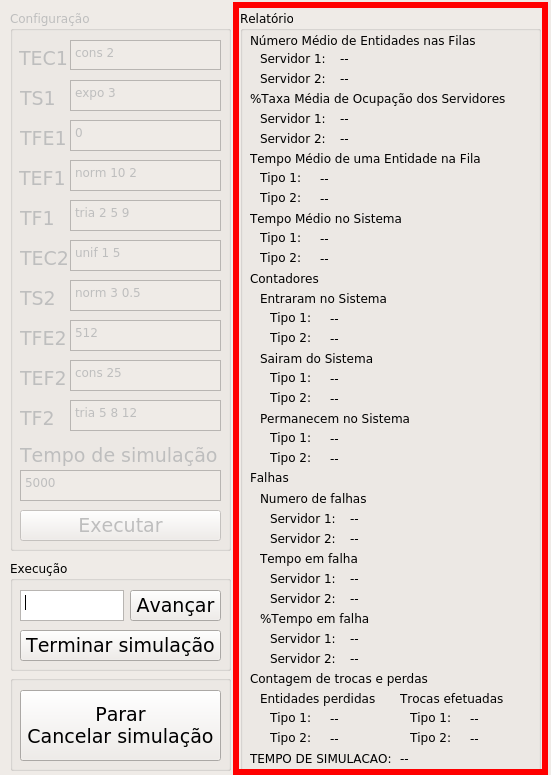
\includegraphics[width=0.4\textwidth]{imgs/rel.png}
\columnbreak

Durante a execução as estatísticas serão mostradas aqui, esse tela será atualizada a cada 
avanço no tempo.

\end{multicols}

\section{Implementação}
A implementação foi feita em \texttt{C++11} utilizando \texttt{Qt} para interface gráfica.

\subsection{Eventos}
A gerencias dos eventos é feita pela classe \texttt{mod::Oraculo}, com os
seguintes atributos:

\begin{itemize}
  \item \texttt{tempo\_}: guarda o tempo atual da simulação
  \item \texttt{tempo\_total}: tempo que a simulação deve terminar.
  \item \texttt{events}, do tipo \texttt{std::multiset<Event>}, guarda os eventos
    ordenados pelo tempo em uma arvore \textit{RB}.
\end{itemize}

Os eventos são da classe \texttt{mod::Event} que contem:
\begin{itemize}
  \item \texttt{time\_}: tempo em que o evento deve ser executado, utilizado para atribuir 
    uma relação de ordem entre os eventos.
  \item \texttt{text}: uma descrição do evento, utilizado para \textit{debugging}.
  \item \texttt{call}: do tipo \texttt{std::function<void()>}, todo evento é um método 
    que recebe e retorna \texttt{void};
\end{itemize}

\subsubsection{Adicionar Evento} 
Para adicionar um evento basta chamar a função \texttt{mod::Oraculo::add\_event} passando o
método que sera chamado no evento (\texttt{F call}), tempo no qual o evento será chamado
(\texttt{double time}) e a descrição do evento (\texttt{std::string text}). O Evento será
criado com esse parâmetros e adiciono em \texttt{events}.

\subsubsection{Executar Eventos}
A função \texttt{mod::Oraculo::run} recebe como argumento o tempo limite de execução
(\texttt{double limit}), os eventos serão chamados em ordem em quanto não estourar
o tempo limite ou o tempo total de execução.

\subsection{Funções de probabilidade}
As funções de probabilidade são geradas pelo método \texttt{mod::parser} que recebe um 
\texttt{std::string} e retorna um \texttt{func::func (Aka std::function<double()>)}. 
A \texttt{std::string text} deve seguir os seguintes padrões:
\begin{itemize}
  \item \texttt{expo media}: Exponencial.
  \item \texttt{norm media dp}: Normal.
  \item \texttt{tria min moda max}: Triangular
  \item \texttt{unif min max} : Uniforme;
  \item \texttt{cons valor}: retorna sempre valor.
\end{itemize}

\subsection{Elementos da modelagem}
Todos elementos da modelagem estão conectados na classe \texttt{Estado}, a baixo segue os
atributos da classe.
\begin{itemize}
  \item \texttt{Entidade}: pode ser do \texttt{Tipo} \texttt{um} ou \texttt{dois}. Não 
    é um atributo da classe \texttt{Estado}, mas é um elemento dinâmico que transita pelo
    sistema. Armazena o tempo em fila e tempo no sistema.
    
    Atributos da classe:
     \begin{itemize}
       \item  \texttt{double begin}: tempo em que a entidade entrou no sistema.
       \item  \texttt{double fila\_begin, fila\_end}: tempo que a entidade entrou e saio da
         fila.
       \item \texttt{Tipo tipo\_}: tipo da entidade.
     \end{itemize}

  \item \texttt{Saida saida}: Remove as Entidades do sistema e responsável pelas
    estatísticas de: \textit{Sairam do Sistema}, \textit{Tempo Médio no Sistema} e
    \textit{Tempo Médio de uma Entidade na Fila}.

    Atributos da classe:
   \begin{itemize}
     \item \texttt{unsigned um, dois}: conta quantas entidades sairão do sistema.
     \item \texttt{double tempo\_um, tempo\_dois}: somatório do tempo de cada entidade 
       que saiu do sistema.
     \item \texttt{double tempo\_em\_fila\_um, tempo\_em\_fila\_dois}: somatório do
       tempo em fila de cada entidade que saiu do sistema.
   \end{itemize}

  \item \texttt{Servidor servidor1, servidor2}: Move as entidades para \texttt{saida} e 
    responsável pelas estatísticas de \textit{Número Médio de Entidades nas Filas},
    \textit{\%Taxa Média de Ocupação dos Servidores}, \textit{Numero de falhas},
    \textit{Tempo em falha} e \textit{\%Tempo em falha}.

    Atributos da classe:
   \begin{itemize}
     \item \texttt{func::func ts, tef, tf}: tempo de serviço, entre falhas e em falha.
     \item \texttt{Saida \&saida}: Referencia para \texttt{saida}.
     \item \texttt{std::queue<Entidade> fila}: fila de entidades.
     \item \texttt{unsigned tfe}: tamanho da fila de entrada.
     \item \texttt{bool em\_falha}: guarda se o servidor esta em falha.
     \item \texttt{unsigned n\_falhas}: contador de falhas do servidor.
     \item \texttt{bool ocupado}: guarda se o servidor esta ocupado.
     \item \texttt{double t\_servico, t\_falha}: tempo total ocupado e em falha.
     \item \texttt{double begin\_ocupado, begin\_falha}: gurda o tempo da ultima vez que, 
       mudou de não ocupado para ocupado e entrou em falha, usado para controle interno.
     \item \texttt{double mfila}: media de Entidades na fila.
     \item \texttt{double ponderacao}: utilizado para calcular a media ponderada de
       Entidades na fila, controle interno.
     \item \texttt{double last\_time}: ultima vez que a media de Entidades na fila foi
       calculada, controle interno.
     \item \texttt{bool init}: utilizado para \texttt{pronderacao} seja atribuída apenas 
       uma vez.
   \end{itemize}

    Eventos:
    \begin{itemize}
      \item \textit{Sair do servidor} que passa um elemento para \texttt{Saida}
        e chama \\\texttt{mod::Servidor::executar\_proximo} que pode gerar o próximo 
        evento \textit{Sair do servidor}. 

      \item \textit{Servidor em falha} coloca o \texttt{Servidor} em modo de falha e
        gera o evento a seguir.

      \item \texttt{Servidor voltou} tira o \texttt{Servidor} de modo de falha, 
        chama \\\texttt{mod::Servidor::executar\_proximo} e, 
        \texttt{mod::Servidor::programar\_falha} para gerar o próximo evento
        \texttt{Servidor em falha}.
    \end{itemize}

  \item \texttt{Chegada chegada1, chegada2}: O \texttt{Estado} possui duas entradas, um
    para cada tipo de entidade. Responsável pela contagem de \textit{Entraram no Sistema}, \textit{Entidades perdidas}  \textit{Trocas efetuadas}.

    Atributos da classe:
   \begin{itemize}
     \item \texttt{func::func tec}: tempo entre chegadas
     \item \texttt{Entidade::Tipo tipo}: tipo de entidade que é gerado
     \item \texttt{Servidor \&primario, \&secundario}: servidor principal e secundário,
       para caso o primeiro não esteja disponível.
     \item \texttt{unsigned entradas, trocas}: contagem de quantas Entidades entraram e quantas foram para o servidor secundário.
     \item \texttt{unsigned perdas}: contagem de quantas Entidades não conseguiram nem entrar na fila do servidor secundário.
   \end{itemize}
 
    Evento:
    \begin{itemize}
      \item \texttt{Evento Chegada}: Tenta adicionar uma entidade no \texttt{Servidor} e 
        gera o próximo \texttt{Evento Chegada}.
    \end{itemize}
\end{itemize}

\subsubsection{Construtor}
O construtor esclarece como as classes são relacionadas.
\lstset{language=C++}  
\begin{lstlisting}[frame=single]  
Estado(std::string tec1, std::string ts1,
       std::string tef1, std::string tf1,
       unsigned tfe1, std::string tec2,
       std::string ts2, std::string tef2,
       std::string tf2, unsigned tfe2,
       double tempo_total)
      :oraculo{tempo_total}, saida{oraculo},
       servidor1{oraculo, func::parse(ts1),
                 func::parse(tef1),
                 func::parse(tf1),
                 saida, tfe1},
       servidor2{oraculo, func::parse(ts2),
                 func::parse(tef2),
                 func::parse(tf2),
                 saida, tfe2},
       chegada1{oraculo, func::parse(tec1),
                Entidade::um, servidor1, servidor2},
       chegada2{oraculo, func::parse(tec2),
                Entidade::dois, servidor2, servidor1}
\end{lstlisting}

\end{document}

